
\chapter{Proposed Method}\label{ch:method}

In this section we dervive anomaly detection method based on spectral decomposition
of time-domain signal.
Our goal is to involve statistical analysis of the frequency components of a 
time-domain signal for detection of the malicious behavior.
%\emph{tunneling protocol} %malicous traffic
%in an application layer as well as 

On the high-frequency scale our method ought to be capable of detection of the
\emph{tunneling protocols} in application layer, while on the very low frequency scale
our method is intended to be capable to detect anomalous behavior in wider time contexts.

Tunneling protocol refer to encapsulation of one network 
protocol in payload of the other. By using tuneling protocol a malicious agent can 
transfer data  belonging to prohibited protocol over a network, bypassing 
a security policies. Our hypotesis is that specific application protocol imprints 
specific pattern in a power spectral density distribution. If the tunneling protocol 
is in use, these patterns are different and anomalous behavior can be detected.

The periodicity can be analyzed on different scales, while tunneling protocol
violates normal pattern on higher frequency scales, we are also concerned about anomalous
patterns in very low frequency scales. This other patterns come up not of violation 
of the standard protocols, but of departure from the typical behavior or the habits. 
E.g. an mallware communicating with the remote server using the HTTP protocol 
does not violate the application protocol. 
But by exchanging information in regular manner, not depending on time of the day,
its behavior will be distint from the behavior of the typical web user who uses the network
in a way, periodic manner.

\name{He et al.} \cite{he2004spectral} showed that the different layers of the network
protocols inprint distinct patterns in a power spectral density distribution. 
Further work of \name{Chen} and \name{Hwang} \cite{chen2007spectral}
used the features derived %TODO use better word
from frequency spectrum to classify malicious and normal traffic.
They noticed that transport protocols (transmission control protocol --
TCP and user datagram protocol - UDP) 
have distinct power spectral density distribution. 
They exploited this property to identify low-rate denial-of-service (DoS)
attacks on TCP protocol. %TODO on TCP protocol?
%an reduction of service (RoS) attacks.
%TODO more writing about features used
\name{Wright et al.} \cite{wright2006inferring} researched methods based on 
hidden Markov models to classify different application protocols embeded in 
encrypted application layer.
They developed classification method, able to classify different 
application protocols multiplexed in single encrypted packet flow.
\name{Dusi et al.} brought an statistical approach 
to detect an tunnel inside application layer.
In  \cite{dusi2009tunnel}  they described different tunneling techniques and designed 
statistical pattern recognition classifier to identify them.

Even though it is not possible to analyze payload of particular packets in 
ecrypted connection, it is possible to observe the time of the packet transit, 
its size, direction, source and destination endpoint, etc. 
This data is denoted as packet traces and it is extracted from unencrypted 
part of the packet. 
The goal is to develop feature creation and pattern recognition method for 
the network packet traces involving spectral analysis.
The method is supposed to detect tunneling protocols only by observation 
of the packet traces.

\section{Data Collection}\label{sec:collect}

The input data for our method consists of a timestamped \emph{packet traces} or a
timestamped \emph{traffic flow} statistics. 

Both can be obtained by capturing
network packet headers. While first one stores each packet (or the packet header)
as a single record,
other one contains total count of the packets and ammount of bytes for 
related sequence of the packets. Relation between packets is determined depending 
on the traffic flow protocol. E.g. for Transmission Control Protocol (TCP) relation is 
determined using following information: capturing interface, source and destination IP address,
source and destination port. 
%
%or Cisco standard \emph{NetFlow}%
%\footnote{
%Cisco standard definest one record (a flow) in Netflow format as a unidirectional sequence of
%packets that share following values: ingress interface; source IP address; destination 
%IP address; IP protocol; source port for UDP or TCP, 0 for other protocols;
%destination port for UDP or TCP, type and code for ICMP, or 0 for other protocols;
%type of service (TOS).
%} 
%protocol. As NetFlow datasets contains only statistics of particular network packet flows, 
%it can be generated from the packet trace data. In practice the NetFlow data is generated by 
%network active components as firewals, routers or swithes. 
%

Due to differences in described formats, we extract following attributes 
from packet trace or traffic flow data in our experiments, 
to allow usage of unified processing methods:
\begin{itemize}
	\item packet or packet flow \emph{timestamp}, i.e. the time when the (first) packet passed
	trought the capturing gateway,
	\item \emph{flow 5-tuple} -- i.e. tranmission \emph{protocol} speciffication and identification of 
	source and destination endpoint
	(e.g. for the TCP or the UDP protocols it is \emph{source address} and \emph{port}, 
	\emph{destination address}  and \emph{port}),
	\item \emph{size} of packet`s payload or \emph{total size} of the packets in case of flow data,
	\item \emph{count} of the packets (for packet trace data it is always one),
	\item \emph{direction}%
	\footnote{%
		We embed \emph{direction information} 
		into the \emph{size} parameter using negative size  
		if packets travel from destination to source and otherwise positive.%
	} %
	with respect to initial packet whithin given flow,
\end{itemize}

We define source endpoint as the endpoint that initiates connection and the destination edpoint 
as the endpoint that  accepts the connection. %TODO what?
Inbound and outbound packets are distinguished
by direction attribude. 

We further require that traffic flow data are allways captured periodically in defined time span.
We can look at this process as a sampling process. We consider the flow capturing period
is lower bound for the sampling period. This can of course cause alliasing as the original
signal contains higher frequency components than the sampling frequency induced by data capturing 
process. For packet trace data there is no upper bound on the sampling frequency induced by 
capturing process, but higher sampling frequency raises the memory and processig time requirements.


\section{Feature Creation}

\subsection{Stochastic process}
% TODO some flesh here

For a specified flow $f$ the packet arrival process $x_f\left[t\right]$ 
(or simply \emph{packet process})  is defined as a count of packet arrivals 
at given timespan $I = \left\langle \frac{t}{s}, \frac{t+1}{s} \right)$:
\begin{equation}\label{packetprocess}
\begin{split}
	 x_f\left[t\right] = \left| 
	\left\lbrace p : f = flow(p) \wedge time(p) \in I \right\rbrace \right|\\
	\forall t \in \mathbb{N}\, ,
\end{split}
\end{equation}
where $s$ is the sample rate, function $flow(p)$  yields the \emph{flow} 5-tuple 
and function $time(p)$  yields the \emph{timestamp} of given packet $p$. 
We can also define packet process for inbound and outbound flows separately:
\begin{equation}\label{xpacketprocess}
\begin{split}
  x_{f,d}\left[t\right] = \left| 
  \left\lbrace p : flow(p) = f \wedge dir(p) = d \wedge time(p) \in I  \right\rbrace \right|\\
  \forall t \in \mathbb{N}\, ,
\end{split}
\end{equation}%
where $dir(p)$ yields a direction of the packet. 

Note that we will refer to single flow and to avoid confusion
we will denote packet process as $x$ and the inbound and
outbound packet processes as $x_{in}$ and $x_{out}$  in equations. 
%\footnote{
%This is very important formula, we need to focus on it; according 
%to \emph{Dusi et al.} \cite{dusi2009tunnel}
%zero-length packets are ulikely to be induced by application, 
%so we can exclude them here; in addition
%they extract incomming and outgoing  stream separately -- 
%I think it is good idea to work with in- and out- streams separately 
%and compute cross-correlation function instead of auto-correlation function.
%The idea of usage I/O cross-correlation function $R_{io}\left(\tau\right)$ 
%instead of auto-correlation is that $R_{io}\left(\tau\right)$ (at the specific 
%time-lag $\tau$) would enforce the typical request-response round-trip. 
%Questionable is, how to physically interpret the resulting spectral components 
%and if the Wiener-Kitchin theorem is applicable.
%}


\subsection{Spectral density estimation}\label{sec:psd}
% TODO some flesh here -  more about wiener-kitchine theorem and sampling theorem

According to a Wiener–Khinchine %TODO reference
theorem the power spectral density $S_{xx}(f)$ (PSD) of the wide-sense stationary 
stochastic process is obtained by application of discrete-time 
Fourier transform $\mathcal{F}_{\cdot}(\omega)$ on autocorrelation function 
of the packet process $R_{xx}\left[\tau\right]$:

\begin{equation}\label{eq:corr}
R_{xx}\left[\tau\right] = E[x\left[t\right]x\left[t+\tau\right]]\, , 
\end{equation}

\begin{equation}\label{eq:psd}
\begin{split}
S_{xx}(\omega) = \mathcal{F}_{R_{xx}}\left(\omega\right) = \sum_{\tau=-\infty}^{\infty} 
\left( R_{xx}\left[\tau\right] \exp\left( -\imath \omega\tau \right)\right) \\ 
\forall f \in \left\langle -\frac{s}{2},\frac{s}{2} \right\rangle\, , 
\end{split}
\end{equation}

where $\tau$ is the time-lag, $E\left[\cdot\right]$ is expected value of a random variable, $\imath$
is the imaginary unit and $\omega$ is the angular frequency $\omega= 2\pi f$. 
%The autocorrelation function is capable of enforcing periodicity. %TODO really?

Analyzing the inbound and outboud packet process can lead to definition of the cross spectral
density\cite{penny2000signal}.
As the power spectral density is Fourier tranform of the autocorrelation function of the 
stochastic process cross spectral density is the fourier transform is the fourier transform
of the cross-correlation function of two stochastic processes. The cross spectral density is
complex as because the cross-correlation function is not symmetric. 
For inbound and outbound packet process we define cross-correlation function $R_{io}$ 
as well as the cross-spectral density $S_{io}$ as follos:

\begin{equation}\label{eq:xcorr}
R_{io}\left[\tau\right] = E[x_{in}\left[t\right]x_{out}\left[t+\tau\right]]\, , 
\end{equation}

\begin{equation}\label{eq:xpsd}
\begin{split}
S_{io}(\omega) = \mathcal{F}_{R_{io}}\left(\omega\right) = \sum_{\tau=-\infty}^{\infty} 
\left( R_{io}\left[\tau\right] \exp\left( -\imath \omega\tau \right)\right) \\ 
\forall f \in \left\langle -\frac{s}{2},\frac{s}{2} \right\rangle\, , 
\end{split}
\end{equation}

Equations (\ref{eq:corr}), (\ref{eq:psd}), (\ref{eq:xcorr}) and (\ref{eq:xpsd}) 
hold under assumption that packet process is \emph{wide-sense stationary random proces}.
This asssumption seems to be false for infinite time span in network traffic.
Furthermore the time span is usually limited to finite number of samples.
For practical reasons we involved an \emph{windowing function} $w(n)$ and 
\emph{discrete Fourier transform} instead of discrete-time Fourier transform. 
The simplest windowing function -- a rectangular windowing is defined as follows:
\begin{equation}
w(n) = \left\lbrace \begin{array}{l} 
1, \mbox{ if } n\in \left\langle 0, M \right) \\ 
0, \mbox{ otherwise} \end{array}\right. \,.
\end{equation}
Windowing function is nonzero inside specified interval $\left\langle 0, M \right)$ 
otherwise it is zero. 
Parameter  $M$ is length of sub-sequence selected from packet arrival proces. 
If the parameter $M$ is too high the packet proces is unlikely to be stationary, 
on the other hand selecting too low value causes spectral leakage, i.e. the energy 
of the main lobe of a spectral response "leaks" to the sidelobes distorting the 
spectral responses \cite{kay1981spectrum} 
(fig.~\ref{fig:leakage_rect_1000},~\ref{fig:leakage_rect_25}). 

\begin{figure}[h!]%
  \centering
        \begin{subfigure}[b]{0.5\textwidth}
                \centering
                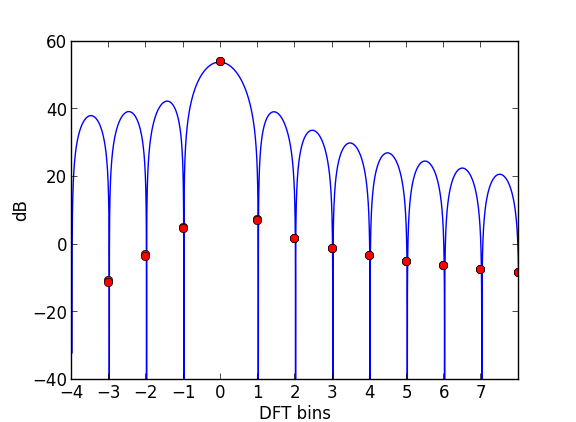
\includegraphics[width=\textwidth]{img/leakage_rect_1000}
                \caption{rectangular, $M=1000$}
                \label{fig:leakage_rect_1000}
        \end{subfigure}%
        ~ \begin{subfigure}[b]{0.5\textwidth}
                \centering
                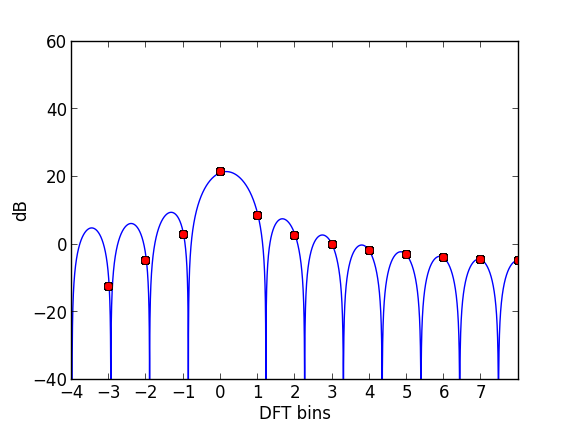
\includegraphics[width=\textwidth]{img/leakage_rect_25}
                \caption{rectangular, $M=25$}
                \label{fig:leakage_rect_25}
        \end{subfigure}%
  \caption{\small Detail of the discrete-time Fourier transform (DTFT) of a sinusoid 
  with rectangular  windowing.
  The unit on x-axis is an Discrete fourier transform (DFT) bin.
  The red dots show values returned by DFT. It is visible that for decreased widow
   size (fig.~\ref{fig:leakage_rect_25}) the distortion is higher.}
  \label{fig:leakage_rect}
\end{figure}

We iteratively apply windowing function to the whole sequence generating 
non-overlapping adjancent sequence of windows. 
We identify the particular window in this sequence with upper index -- 
e.g. $S_{xx}^i$ is a power spectral density function of an $i$-th window.
Thus, we rewrite equations (\ref{eq:corr}) and (\ref{eq:psd}) for non-overlapping 
windows as follows:
\begin{equation}\label{eq:corr2}
R_{xx}^i\left[m\right] = \frac{1}{M} \sum_{t=0}^{M}
 x\left[t+iM\right]x\left[t+m+iM\right] \, , 
\end{equation}
\begin{equation}\label{eq:psd2}
\begin{split}
S_{xx}^i(k) = \mathcal{F}_{R_{xx}^i}\left(k\right) = \sum_{m=0}^{M-1}
\left( R_{xx}^i \left[m\right] w(m) \exp\left( -\imath 2\pi m\frac{k}{M} \right)\right)\\
\forall k \in \left\{ 0,1,2,...,M-1 \right\}\, . 
\end{split}
\end{equation}
and similarly for cross spectral density:
\begin{equation}\label{eq:xcorr2}
R_{io}^i\left[m\right] = \frac{1}{M} \sum_{t=0}^{M} 
 x_{in}\left[t+iM\right]x_{out}\left[t+m+iM\right] \, , 
\end{equation}
\begin{equation}\label{eq:xpsd2}
\begin{split}
S_{io}^i(k) = \mathcal{F}_{R_{io}^i}\left(k\right) = \sum_{m=0}^{M-1}
\left( R_{io}^i \left[m\right] w(m) \exp\left( -\imath 2\pi m\frac{k}{M} \right)\right)\\
\forall k \in \left\{ 0,1,2,...,M-1 \right\}\, . 
\end{split}
\end{equation}
Note that the windowing function is inherent in equations (\ref{eq:corr2}) and (\ref{eq:psd2})
by using limitted ranges of sumation, and domain of definition of the power spectral density.

\begin{figure}[h!]%
  \centering
        \begin{subfigure}[b]{0.5\textwidth}e
                \centering
                \includegraphics[width=\textwidth]{img/leakage_hamming_1000}
                \caption{hamming, $M=1000$}
                \label{fig:leakage_hamming_1000}
        \end{subfigure}%
        ~ \begin{subfigure}[b]{0.5\textwidth}
                \centering
                \includegraphics[width=\textwidth]{img/leakage_hamming_25}
                \caption{hamming, $M=25$}
                \label{fig:leakage_hamming_25}
        \end{subfigure}%
  \caption{\small Detail of the discrete-time Fourier transform (DTFT) of a sinusoid 
  with hamming windowing.
  The unit on x-axis is an Discrete fourier transform (DFT) bin.
  The red dots show values returned by DFT. It is visible that for decreased widow
   size (fig.~\ref{fig:leakage_hamming_25}) the distortion is higher.}
  \label{fig:leakage_hamming}
\end{figure}

By involving windowing function we introduced
\emph{spectral leakge}. Use of apodization function, e.g. \emph{Hamming} %TODO explain 
(see fig.~\ref{fig:leakage_hamming_1000} and \ref{fig:leakage_hamming_25}),
%or \emph{Hamming} (\ref{eq:hamm}) 
could be appropiate in decreasing leakage:
%\begin{equation}\label{eq:hann}
%w(n) = \left\lbrace \begin{array}{l} 
%0.5\left(1 - \cos \left ( \frac{2 \pi n}{N-1} \right) \right), \mbox{ if } n\in \left\langle 
%0, M \right) \\ 0, \mbox{ otherwise} \end{array}\right. \,.
%\end{equation}
\begin{equation}\label{eq:hamm}
w(n) = \left\lbrace \begin{array}{l} 
0.54 - 0.46\cos \left ( \frac{2\pi n}{N-1} \right), \mbox{ if } n\in \left\langle 0, M \right) \\
 0, \mbox{ otherwise} \end{array}\right. \,.
\end{equation}
The hamming window still allows to leak the power to nearby DFT bins as the
main lobe is wider, but the attenuation of in side lobes is higher.
Even the hamming window cannot provide good results for the low values of the $M$ 
parameter. In addition there is allways tradeoff between effective bandwidth and
sidelobe attenuation. \name{Yoon} et al. \cite{yoon2009butterworth} windowing technique 
involving a Buttleworth filter to overcome the problems with reduction of bandwith 
while elevating sidelobe attenuation.

The sampling rate $s$ must be selected according to the Nyquist theorem. 
Too low value entails aliasing%
\footnote{
    The aliasing is caused by folding of the frequencies above Nyquist frequency
    $\frac{s}{2}$ symmetrically below this frequency. 
    To properly reconstruct the signal that contain no frequency higher than $f_{max}$ 
    the sample rate is bounded by $s > 2f_{max}$.
}%
, while too high value incurs data storage and processing overhead. 

%\subsection{Pattern definition}
By application of the Fourier transform original features has been mapped into new space.
We denote features in new space as \emph{spectral components} (or \emph{frequency components}).
Temporal context of the features has been altered. 
In new feature space the temporal context is determined by sequence
of the detection windows of size $M$. 
%At the level of the detection window a temporal notion is decomposed 
%into tuple of temporal functions parametrised by \emph{spectral components}.

The determination of the changes in spectrum in local time context is related to short-term
Fourier analysis or short-term Fourier transform. Whereas this approach introduces
resolution problems wavelet transform or multiresolutional analysis can be used for
time-frequency analysis. We are not concerned with temporal context at this point.
Although temporal aspect is still present it has not been used in further analysis 
in present work. Anomalies in new feature space are thus regarded to as \emph{point anomalies}. 

\subsection{Summary}

There are few parameters affecting quality of the  features: %TODO what?
the sample rate $s$ and the window length $M$. 
In addition, \emph{spectral components} can be subject to further feature extraction 
comprising combination of extisting features or discarding irrelevant, 
redundant  or noisy%
\footnote{
    In case of low signal-to-noise ratio, a feature is typically not usefull 
    for discriminative outcome.
} %
ones using data-mining methods or based on the empirical domain knowledge.

This aspects and process of seeking of proper parameters are subject of further 
research and they are discussed in \emph{chapter \ref{sec:experiments}}.

\section{Model Estimation and Anomaly Detection}

In order to detect anomalies a model of normal or anomalous behavior or even both
must be constructed. The naive approach is to estimate an multivariate gaussian 
model under assumption of \emph{central limit theorem}. This approach encounters 
serveral problems. The most notable is the curse of dimensionality - 
an phenomena occuring when analyzing data in high-dimensional spaces.
The statistical view on this problem is that by applying tranformations 
to increase dimensionality the data becomes sparse. It is problem to 
have statisticaly significat outcome as the amount data needed is emerging
exponentially with dimensionality. Of course usage of exponentially larger

Another facet of mentioned naive approach is assuption of central limit theorem, 
meaning that the data instances are independent and identically distributed. 
In addition, to obtain an sound and reliable result sufficient number of data instances 
must be present. This is often problem as the data instances that are related to anomalies 
are less common in data. Additional data instances can be artificially simulated in order 
to enable ability to construct an reliable model. Introducing  systmatic errors during 
simulation can lead to biased model estimator. %In addition simulation of annomalous
%intances can bias the model as it affects the extent in which are such instances present in data.

The solution to course of dimensionality is to reduce dimensionality of the feature space.
This can refer to finding manifold of denser data in original sparse feature space.
Reduction of dimensionality is then proces of estimation of topological properties of such 
manifold and the estimation of relations between data instances on the topological surface. 
Another approach is to use empirical domain knowledge to infer relations in the
data to perform transformation in lower dimansional space.

Spectral density of a signal in time domain represents continous decomposition of signal to
periodic components present in the original signal. Altought it is continous function in
practice only estimations are available. In section \ref{sec:psd} we derived descrete estimator
based on auto-correlation function. The analyzed signal is connected to stochastic processes
that occur in computer network. The frequency distribution of signals in such a system is 
affected by many attributes. Our assumption is that te stochastic processs in computer network
are not dynamic. It is false thougth to try to pick an specific characteristic frequency component
and treat it as a discriminative feature for specific undelaying process. As example already 
explored by \name{He} et al. \cite{he2004spectral} when an saturated link is changing its 
speed the characteristic frequency changes as well.

\name{Chen} et al. \cite{chen2007tcp} presented an apaproach where modeled distribution
of a standard deviation over spectral densities and also multivariate distribution over
frequency bands. Their model used diagonal covariance matrix. They performed hypotesis 
testing in order to classify an cut off specific type of denial-of-service (DoS) attacks.

In present work we consider both methods of statistical analysis of the spectral density as feasible.
In our approach we involve multivariate Gaussian distribution to construct the model 
and Mahalanobis distance to measure deviation of the tested samples from the model.

\subsection{Feature Extraction}

The fourier transform of the autocorrelation function is real and symmetric.
 The reason is that periods in input data turn into positive and negative
components. As negative components contains same information as the postive they 
can be discarded. We also discard zero component.

Let us denote the unbiased estimator of the variance of the spectral density

\begin{equation}\label{eq:sdev}
\begin{split}
s^i = \sqrt{ \frac{1}{\frac{M}{2}-2} \sum_{k=1}^{\frac{M}{2}-1} \left( S_{xx}^i\left(k\right) - 
\overline{S_{xx}^i} \right)^2 }  \, , 
\end{split}
\end{equation}
where $\overline{S_{xx}^i} $ is the mean value of the obserations and $M$ is the
count of the spectral comoponents. First half are posive components.


%TODO frequency bands and multivariate gaussian distribution

\subsection{Model Estimation}

\section{Assessment and Interpretation of Results}
